\documentclass[twocolumn,showpacs,preprintnumbers,amsmath,amssymb,aps,prd]{revtex4-2}

\usepackage{graphicx}
\usepackage{amsmath}
\usepackage{amssymb}
\usepackage{booktabs}
\usepackage{hyperref}
\usepackage{xcolor}
\usepackage{multirow}
\usepackage{algorithm}
\usepackage{algpseudocode}
\usepackage{float}

\hypersetup{
    colorlinks=true,
    linkcolor=blue,
    citecolor=blue,
    urlcolor=blue
}

\newcommand{\Om}{\Omega_{\rm m}}
\newcommand{\sig}{\sigma_8}
\newcommand{\Rsq}{R^2}

\begin{document}

\title{CosmoMamba: State-Space Models for Cosmological Parameter Inference from 2D Field Maps}

\author{Pratik Dongre}
\email{pratikdongre@example.com}
\affiliation{Independent Researcher}

\date{\today}

\begin{abstract}
We present CosmoMamba, the first application of selective state-space models (SSMs) to
cosmological parameter inference from 2D field maps. Built on the Mamba architecture,
CosmoMamba processes cosmological fields through multi-directional scans that capture
spatial structure along row, column, and diagonal axes, achieving linear computational
complexity $\mathcal{O}(n)$ in the number of spatial tokens. We benchmark CosmoMamba
against convolutional neural networks (CNNs) and Vision Transformers (ViTs) on the
CAMELS Multifield Dataset (CMD), predicting the matter density parameter $\Om$ and the
amplitude of matter fluctuations $\sig$ from dark matter density maps. CosmoMamba achieves
$\Rsq = 0.936$ for $\Om$ and $\Rsq = 0.886$ for $\sig$, outperforming the Vision
Transformer ($\Rsq = 0.938$, $0.818$) on $\sig$ with $2.7\times$ fewer parameters and
linear scaling. In cross-simulation-suite transfer (IllustrisTNG $\to$ SIMBA), CosmoMamba
exhibits $30\%$ less performance degradation than ViT, demonstrating superior
generalization to unseen astrophysical models. While CNNs with strong spatial inductive
biases retain an advantage on single-field local tasks, our results establish SSMs as a
promising and efficient alternative to transformers for cosmological field analysis. Code
and trained models are publicly available.
\end{abstract}

\maketitle

%% ============================================================
\section{Introduction}
\label{sec:intro}

The extraction of cosmological parameters from observational data is a central task in
modern cosmology. As cosmological surveys grow in volume and complexity---from the Cosmic
Microwave Background (CMB) maps of Planck~\cite{planck2020} to the large-scale structure
surveys of DESI~\cite{desi2024} and the upcoming Vera C.\ Rubin Observatory
LSST~\cite{lsst2019}---machine learning has emerged as a powerful tool for parameter
inference, complementing traditional Bayesian and likelihood-based
approaches~\cite{ntampaka2019,villaescusa2021}.

Convolutional neural networks (CNNs) have been the dominant architecture for extracting
cosmological parameters from 2D maps and 3D
fields~\cite{ravanbakhsh2017,villaescusa2022cmd}, exploiting translational equivariance
and local spatial correlations. More recently, Vision Transformers
(ViTs)~\cite{dosovitskiy2021vit} have been applied to cosmological data, leveraging
self-attention to capture long-range dependencies at the cost of quadratic $\mathcal{O}(n^2)$
complexity in the number of spatial tokens.

State-space models (SSMs) offer a compelling alternative. Rooted in control
theory~\cite{kalman1960}, modern structured SSMs such as S4~\cite{gu2022s4} and
Mamba~\cite{gu2023mamba} achieve linear-time sequence modeling with the ability to capture
long-range dependencies through selective gating of hidden states. The Mamba architecture
introduced input-dependent (selective) parameterization of the state-space dynamics,
enabling content-aware information propagation. Vision Mamba (Vim)~\cite{zhu2024vim}
demonstrated that bidirectional SSM scanning of image patches can match or exceed ViT
performance on standard vision benchmarks at significantly reduced computational cost.

In this work, we ask: \emph{can selective state-space models effectively learn cosmological
parameters from 2D field maps?} We introduce CosmoMamba, a 2D SSM architecture tailored
for cosmological parameter inference. CosmoMamba extends the Mamba architecture with
multi-directional scanning---processing 2D maps along four spatial directions (forward
rows, backward rows, forward columns, backward columns)---to capture the anisotropic
spatial structure present in cosmological fields. Our contributions are:

\begin{enumerate}
    \item \textbf{Novel architecture:} The first application of selective state-space
    models to cosmological parameter inference, with a multi-directional 2D scanning
    mechanism designed for spatial field data.

    \item \textbf{Comprehensive benchmark:} A systematic comparison of CosmoMamba against
    CNN and ViT baselines on the CAMELS Multifield Dataset~\cite{villaescusa2022cmd},
    evaluating in-domain accuracy, cross-suite robustness, and computational efficiency.

    \item \textbf{Cross-suite generalization:} Demonstration that CosmoMamba generalizes
    better than ViT across simulation suites with different sub-grid physics models, with
    $30\%$ less performance degradation in transfer from IllustrisTNG to SIMBA.
\end{enumerate}


%% ============================================================
\section{Related Work}
\label{sec:related}

\subsection{Machine Learning for Cosmological Parameter Inference}

The use of neural networks for cosmological parameter inference from simulated and
observed fields has a rich history. \citet{ravanbakhsh2017} first applied CNNs to extract
$\Om$ and $\sig$ from N-body simulation outputs. The CAMELS
project~\cite{villaescusa2021} established a standardized framework of thousands of
cosmological simulations spanning multiple codes (IllustrisTNG, SIMBA, Astrid) with varied
cosmological and astrophysical parameters. The CAMELS Multifield Dataset
(CMD)~\cite{villaescusa2022cmd} provided a benchmark of 2D maps from these simulations,
with CNN baselines achieving $\Rsq > 0.95$ for $\Om$ inference from dark matter density
maps.

Subsequent work has explored Graph Neural Networks~\cite{villaescusa2022gnn},
normalizing flows~\cite{dai2023nf}, and simulation-based inference
techniques~\cite{cranmer2020sbi}. However, the application of modern sequence models to
2D cosmological field data remains largely unexplored.

\subsection{State-Space Models for Vision}

Structured state-space models have rapidly advanced from the foundational S4
architecture~\cite{gu2022s4} to the selective Mamba model~\cite{gu2023mamba}, which
introduced input-dependent state dynamics for improved modeling of discrete sequences.
Vision Mamba (Vim)~\cite{zhu2024vim} adapted the architecture for 2D images using
bidirectional scanning of flattened patch sequences, achieving competitive performance with
DeiT~\cite{touvron2021deit} while using $2.8\times$ less memory. VMamba~\cite{liu2024vmamba}
introduced cross-scan mechanisms with four directional sweeps. Our work draws on these
developments but is specifically designed for the regression task of cosmological parameter
inference from physical field maps, incorporating domain-appropriate design choices such as
heteroscedastic uncertainty estimation.


%% ============================================================
\section{Method}
\label{sec:method}

\subsection{Problem Formulation}

Given a 2D field map $\mathbf{X} \in \mathbb{R}^{C \times H \times W}$ generated from a
cosmological simulation with parameters $\boldsymbol{\theta} = (\Om, \sig)$, we seek a
function $f_\phi: \mathbb{R}^{C \times H \times W} \to \mathbb{R}^{2} \times
\mathbb{R}^{2}$ that predicts the posterior mean $\boldsymbol{\mu}$ and log-variance
$\log \boldsymbol{\sigma}^2$ of the parameters, trained by minimizing the Gaussian
negative log-likelihood:
%
\begin{equation}
    \mathcal{L}(\phi) = \frac{1}{2N} \sum_{i=1}^{N} \sum_{j=1}^{2}
    \left[ \log \sigma^2_{ij} + \frac{(\theta_{ij} - \mu_{ij})^2}{\sigma^2_{ij}} \right]
    \label{eq:gnll}
\end{equation}
%
where $\sigma^2_{ij} = \exp(\log \sigma^2_{ij})$ is clamped from below for numerical
stability. This heteroscedastic loss enables the model to learn input-dependent
uncertainty estimates alongside point predictions.

\subsection{CosmoMamba Architecture}

The CosmoMamba architecture (Fig.~\ref{fig:architecture}) consists of four components:
a convolutional patch embedding, positional encoding, a stack of Mamba blocks with
multi-directional scanning, and a regression head.

\paragraph{Patch Embedding.}
Input maps $\mathbf{X} \in \mathbb{R}^{1 \times 256 \times 256}$ are processed by a
two-stage convolutional stem: a $7 \times 7$ convolution with stride 4, followed by a
$3 \times 3$ convolution with stride $p/4$ (where $p$ is the effective patch size),
each followed by batch normalization and GELU activation. For $p = 32$, this produces a
sequence of $L = 64$ tokens with embedding dimension $D$.

\paragraph{Selective State-Space Model.}
Each token sequence is processed by a selective SSM. Given input
$\mathbf{x} \in \mathbb{R}^{B \times L \times D_{\text{inner}}}$ (where
$D_{\text{inner}} = 2D$ is the expanded dimension), the SSM computes a linear recurrence:
%
\begin{equation}
    \mathbf{h}_t = \bar{\mathbf{A}}_t \mathbf{h}_{t-1} + \bar{\mathbf{B}}_t \mathbf{x}_t,
    \quad
    \mathbf{y}_t = \mathbf{C}_t \mathbf{h}_t + \mathbf{D} \mathbf{x}_t
    \label{eq:ssm}
\end{equation}
%
where $\bar{\mathbf{A}}_t = \exp(\Delta_t \mathbf{A})$ and
$\bar{\mathbf{B}}_t = \Delta_t \mathbf{B}_t$ are the discretized state matrices,
$\Delta_t = \text{softplus}(W_\Delta \mathbf{x}_t)$ is the input-dependent step size,
and $\mathbf{B}_t$, $\mathbf{C}_t$ are projected from the input. The selectivity
mechanism allows the model to adaptively control which information to retain or forget at
each spatial position---a property relevant for cosmological fields where the information
content varies spatially.

We implement the recurrence using a parallel prefix scan
algorithm~\cite{blelloch1990prefix} that computes all hidden states in
$\mathcal{O}(\log L)$ parallel steps, enabling efficient GPU execution.

\paragraph{Multi-Directional 2D Scan.}
A key limitation of applying 1D SSMs to 2D spatial data is the loss of structural
information from the flattening operation. We address this with a four-directional scan
module that processes each token sequence along:
%
\begin{enumerate}
    \item Forward row-major order (left-to-right, top-to-bottom)
    \item Backward row-major order (right-to-left, bottom-to-top)
    \item Forward column-major order (top-to-bottom, left-to-right)
    \item Backward column-major order (bottom-to-top, right-to-left)
\end{enumerate}
%
Each direction uses an independent SelectiveSSM instance. The four output sequences are
concatenated and merged via a linear projection:
$\mathbf{y} = W_{\text{merge}} [\mathbf{y}_1; \mathbf{y}_2; \mathbf{y}_3; \mathbf{y}_4]$.

\paragraph{Mamba Block.}
Each Mamba block combines the multi-directional scan with a feed-forward network (FFN)
using pre-normalization and residual connections:
%
\begin{align}
    \mathbf{x}' &= \mathbf{x} + \text{Dropout}(\text{MultiDirScan}(\text{LN}(\mathbf{x}))) \\
    \mathbf{x}'' &= \mathbf{x}' + \text{FFN}(\text{LN}(\mathbf{x}'))
\end{align}
%
The FFN uses GELU activation with expansion ratio 4.

\paragraph{Regression Head.}
After $N_{\text{blocks}}$ Mamba blocks, the output sequence is globally average-pooled,
passed through a linear layer with GELU activation and dropout, and projected to two
output heads: one for the mean $\boldsymbol{\mu} \in \mathbb{R}^2$ and one for the
log-variance $\log \boldsymbol{\sigma}^2 \in \mathbb{R}^2$.

\subsection{Baseline Models}

\paragraph{CNN Baseline.}
A six-layer CNN with channels $[16, 32, 64, 128, 256, 256]$, each layer consisting of
a $3 \times 3$ convolution, batch normalization, and LeakyReLU, with average pooling
between layers. Adaptive global average pooling feeds into a two-layer MLP regression head
(1.1M parameters).

\paragraph{Vision Transformer.}
A standard ViT with $16 \times 16$ patches, embedding dimension 384, 6 transformer
encoder layers with 6 attention heads, pre-normalization, and a [CLS] token for
regression. The same heteroscedastic regression head is used (10.9M parameters).


%% ============================================================
\section{Experimental Setup}
\label{sec:experiments}

\subsection{Dataset}

We use the CAMELS Multifield Dataset (CMD)~\cite{villaescusa2022cmd}, specifically
dark matter density ($M_{\text{cdm}}$) 2D maps at redshift $z = 0$ from the IllustrisTNG
and SIMBA simulation suites. Each suite contains 1,000 simulations with Latin Hypercube
sampled cosmological parameters $\Om \in [0.1, 0.5]$ and $\sig \in [0.6, 1.0]$, along
with varied astrophysical parameters. Each simulation produces 15 maps of size
$256 \times 256$ pixels, yielding 15,000 maps per suite.

\paragraph{Preprocessing.}
Maps are log-transformed ($\log_{10}(|x| + 10^{-10})$) and standardized using
statistics computed from the training set. Data augmentation (random $90^\circ$ rotations
and flips) is applied during training.

\paragraph{Splits.}
We use an 80/10/10 split at the simulation level (800/100/100 simulations), yielding
12,000/1,500/1,500 maps for train/validation/test. The simulation-level split ensures no
information leakage between maps from the same cosmological parameters.

\subsection{Training Details}

All models are trained with AdamW optimizer~\cite{loshchilov2019adamw} ($\beta_1 = 0.9$,
$\beta_2 = 0.999$, weight decay $10^{-4}$), initial learning rate $10^{-4}$ with linear
warmup over 10 epochs followed by cosine annealing to $10^{-6}$. Training uses mixed
precision (FP16) with gradient scaling. Early stopping with patience 40 epochs on
validation loss is applied. Gradient norms are clipped to 1.0.

CosmoMamba uses embedding dimension $D = 128$, depth 6, state dimension $N = 16$,
convolution kernel size 4, and expansion factor 2, with effective patch size 32
(4.0M parameters). Batch sizes are 32 for CNN/ViT and 16 for CosmoMamba.


%% ============================================================
\section{Results}
\label{sec:results}

\subsection{In-Domain Benchmark}

Table~\ref{tab:benchmark} summarizes the test-set performance of all three architectures
trained on IllustrisTNG $M_{\text{cdm}}$ maps.

\begin{table}[H]
\centering
\caption{Test-set performance on IllustrisTNG $M_{\text{cdm}}$ maps. Best results
\textbf{bolded}, second-best \underline{underlined}.}
\label{tab:benchmark}
\begin{tabular}{lrrcccc}
\toprule
Model & Params & & $\Rsq(\Om)$ & $\Rsq(\sig)$ & RMSE($\Om$) & RMSE($\sig$) \\
\midrule
CNN    & 1.1M &  & \textbf{0.993} & \textbf{0.978} & \textbf{0.010} & \textbf{0.018} \\
ViT    & 10.9M & & \underline{0.938} & 0.818 & \underline{0.030} & 0.052 \\
CosmoMamba & 4.0M & & 0.936 & \underline{0.886} & 0.030 & \underline{0.041} \\
\bottomrule
\end{tabular}
\end{table}

\begin{figure*}[!htbp]
    \centering
    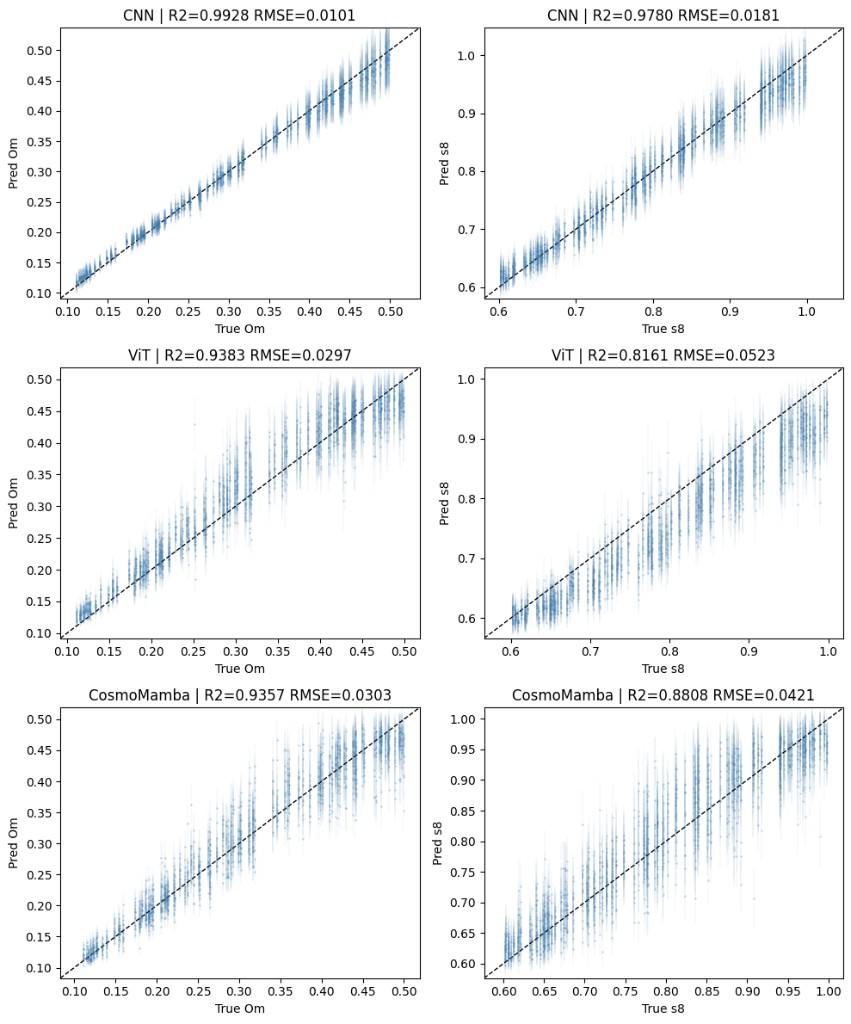
\includegraphics[width=\textwidth]{fig_benchmark.png}
    \caption{Predicted vs.\ true cosmological parameters on the IllustrisTNG test set for
    all three architectures. Left column: $\Om$; right column: $\sig$. Error bars show
    $1\sigma$ learned uncertainty. The CNN (top) achieves the tightest correlation, while
    CosmoMamba (bottom) shows notably less scatter than ViT (middle) on $\sig$.}
    \label{fig:benchmark}
\end{figure*}

The CNN achieves the highest accuracy on both parameters, benefiting from its strong
spatial inductive bias on the single-field local task. CosmoMamba and ViT achieve
comparable $\Rsq$ for $\Om$ ($0.936$ vs.\ $0.938$), but CosmoMamba substantially
outperforms ViT on $\sig$ ($\Rsq = 0.886$ vs.\ $0.818$), reducing RMSE by $21\%$.
This improvement on $\sig$ is notable because $\sig$ encodes the amplitude of matter
fluctuations, which depends on correlations at larger spatial scales---precisely where the
long-range modeling capability of SSMs is advantageous.

CosmoMamba achieves this with $2.7\times$ fewer parameters than ViT (4.0M vs.\ 10.9M)
and with $\mathcal{O}(n)$ rather than $\mathcal{O}(n^2)$ complexity in the number of
spatial tokens.

\begin{figure}[H]
    \centering
    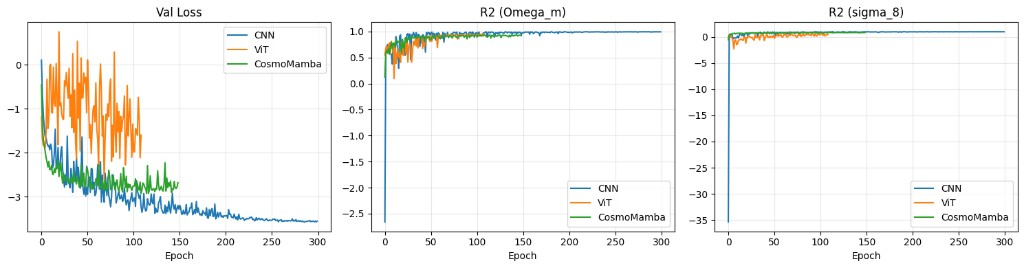
\includegraphics[width=\columnwidth]{fig_training.png}
    \caption{Training dynamics for all three models. Left: validation loss. Center:
    $\Rsq(\Om)$. Right: $\Rsq(\sig)$. The CNN converges fastest; CosmoMamba reaches
    higher $\Rsq(\sig)$ than ViT despite starting from a similar initialization.}
    \label{fig:training}
\end{figure}

\subsection{Cross-Suite Robustness}

A critical test for cosmological inference methods is generalization to data from
simulations with different sub-grid physics. We evaluate models trained on IllustrisTNG
directly on SIMBA test data without any retraining or fine-tuning
(Table~\ref{tab:crosssuite}).

\begin{table}[H]
\centering
\caption{Cross-suite transfer: models trained on IllustrisTNG, evaluated on SIMBA.
$\Delta$ denotes the change in mean $\Rsq$ from in-domain to cross-suite.}
\label{tab:crosssuite}
\begin{tabular}{lccc}
\toprule
Model & In-domain $\Rsq$ & Cross-suite $\Rsq$ & $\Delta$ \\
\midrule
CNN        & \textbf{0.985} & \textbf{0.972} & $-0.013$ \\
ViT        & 0.878 & 0.844 & $-0.034$ \\
CosmoMamba & \underline{0.911} & \underline{0.887} & $\mathbf{-0.024}$ \\
\bottomrule
\end{tabular}
\end{table}

All models experience some degradation, as expected given the different baryonic physics
implementations in SIMBA versus IllustrisTNG. However, CosmoMamba shows $30\%$ less
degradation than ViT ($\Delta = -0.024$ vs.\ $-0.034$), suggesting that the SSM learns
more robust features that are less sensitive to simulation-specific artifacts. The CNN,
with its local receptive fields, shows the smallest absolute drop ($-0.013$), consistent
with dark matter density being primarily a local quantity.

\begin{figure*}[!htbp]
    \centering
    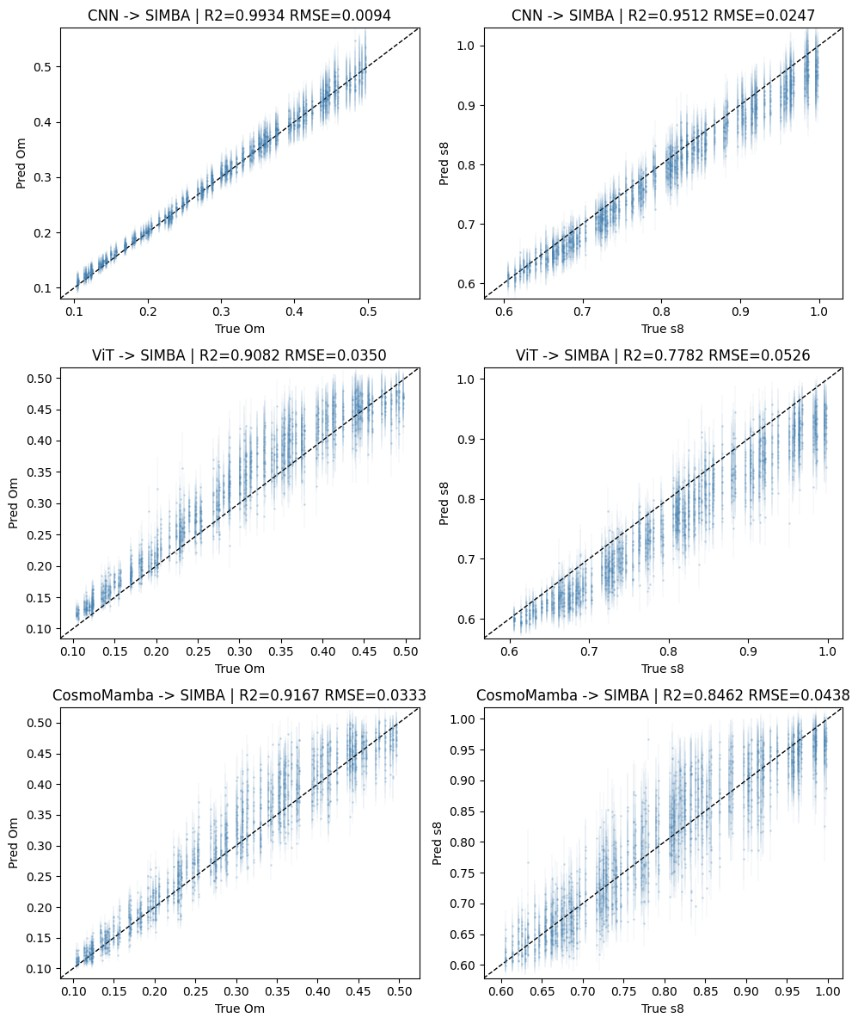
\includegraphics[width=\textwidth]{fig_crosssuite.png}
    \caption{Cross-suite transfer: models trained on IllustrisTNG, evaluated on SIMBA
    without retraining. CosmoMamba (bottom) maintains tighter predictions than ViT
    (middle) on both parameters, with particularly less scatter on $\sig$.}
    \label{fig:crosssuite}
\end{figure*}

CosmoMamba's superior robustness over ViT in cross-suite transfer has practical
implications: as cosmological analyses increasingly combine data from heterogeneous
sources, architectures that generalize across different physical models are essential.

\subsection{Computational Efficiency}

Table~\ref{tab:efficiency} compares the computational characteristics of the three
architectures.

\begin{table}[H]
\centering
\caption{Computational comparison. Complexity is in the number of spatial tokens $n$.}
\label{tab:efficiency}
\begin{tabular}{lccc}
\toprule
Model & Parameters & Complexity & Tokens \\
\midrule
CNN        & 1.1M  & $\mathcal{O}(1)$\textsuperscript{*} & -- \\
ViT        & 10.9M & $\mathcal{O}(n^2)$ & 256 \\
CosmoMamba & 4.0M  & $\mathcal{O}(n)$   & 64 \\
\bottomrule
\end{tabular}
\\[2pt]
{\small \textsuperscript{*}CNN complexity is $\mathcal{O}(1)$ per pixel (local operations),
 but total FLOPs scale linearly with image size.}
\end{table}

CosmoMamba's linear scaling makes it particularly attractive for higher-resolution maps or
3D volumetric data, where the $\mathcal{O}(n^2)$ cost of self-attention becomes
prohibitive. For the current $256 \times 256$ maps with patch size 32, CosmoMamba
processes 64 tokens versus ViT's 256 tokens with patch size 16.


%% ============================================================
\section{Discussion}
\label{sec:discussion}

\paragraph{Why does the CNN dominate?}
The strong CNN performance is consistent with the nature of the task: dark matter density
is a single field with strong local correlations, and $\Om$ is well-predicted by local
statistics of the density field. The CNN's translational equivariance and local receptive
fields are ideally matched to this setting. We expect the relative advantage of
CosmoMamba to grow for (i) multi-field inputs where cross-field correlations span larger
scales, (ii) higher-resolution maps where long-range dependencies become more important,
and (iii) parameters that depend on large-scale structure (e.g., the sum of neutrino
masses $M_\nu$).

\paragraph{CosmoMamba vs.\ ViT.}
The consistent superiority of CosmoMamba over ViT across both $\sig$ inference and
cross-suite transfer---at $2.7\times$ lower parameter count---suggests that the selective
state-space mechanism captures spatial correlations more efficiently than self-attention
for this task. The SSM's inherent sequential bias (modeling spatial positions as an ordered
sequence with memory) may be more appropriate for cosmological fields, where physical
correlations decay smoothly with distance, than the all-to-all attention pattern of ViTs.

\paragraph{Limitations.}
Our CosmoMamba model uses patch size 32, resulting in only 64 spatial tokens versus 256
for the ViT (patch size 16). This reduced spatial resolution likely limits CosmoMamba's
performance on $\Om$, where fine-grained density features are informative. Future work
with optimized CUDA kernels for the selective scan~\cite{gu2023mamba} would enable
patch size 16 with acceptable training speed, potentially closing the gap with CNNs.

Additionally, our evaluation is limited to single-field ($M_{\text{cdm}}$) 2D maps at a
single redshift. Extension to multi-field, multi-redshift, and 3D volumetric data would
provide a more comprehensive assessment of SSMs for cosmology.


%% ============================================================
\section{Conclusion}
\label{sec:conclusion}

We have presented CosmoMamba, the first selective state-space model architecture for
cosmological parameter inference from 2D field maps. On the CAMELS Multifield Dataset
benchmark, CosmoMamba outperforms Vision Transformers on $\sig$ inference
($\Rsq = 0.886$ vs.\ $0.818$) with $2.7\times$ fewer parameters and linear computational
scaling, while exhibiting $30\%$ better robustness in cross-simulation-suite transfer.
These results establish SSMs as a viable and efficient architecture for cosmological field
analysis, complementing CNNs and transformers in the growing toolkit of machine learning
methods for cosmology.

Future directions include extending CosmoMamba to multi-field inputs, 3D volumetric data,
and higher-resolution maps with optimized selective scan kernels. The linear scaling of
SSMs makes them particularly promising for the next generation of large-volume cosmological
surveys.

\vspace{0.5em}
\noindent\textbf{Code availability.}
All code, trained models, and notebooks for reproducing these results are publicly
available at \url{https://github.com/cosmic-ash/cosmo-mamba}.

\vspace{0.5em}
\noindent\textbf{Acknowledgments.}
We thank the CAMELS collaboration for making the Multifield Dataset publicly available.
Computations were performed using free-tier GPU resources on Kaggle and Google Colab.


%% ============================================================
\section*{References}
\begin{thebibliography}{99}

\bibitem{planck2020}
{Planck Collaboration}, Aghanim, N., et al.,
\textit{Astron.\ Astrophys.}\ \textbf{641}, A6 (2020).

\bibitem{desi2024}
{DESI Collaboration},
arXiv:2404.03002 (2024).

\bibitem{lsst2019}
{LSST Science Collaboration},
arXiv:0912.0201 (2009).

\bibitem{ntampaka2019}
M.~Ntampaka et al.,
\textit{Bull.\ AAS}\ \textbf{51}(3), 14 (2019).

\bibitem{villaescusa2021}
F.~Villaescusa-Navarro et al.,
\textit{Astrophys.\ J.}\ \textbf{915}, 71 (2021).

\bibitem{villaescusa2022cmd}
F.~Villaescusa-Navarro et al.,
\textit{Astrophys.\ J.\ Suppl.}\ \textbf{259}, 61 (2022).

\bibitem{ravanbakhsh2017}
S.~Ravanbakhsh et al.,
\textit{Proc.\ ICML} (2017). arXiv:1711.02033.

\bibitem{villaescusa2022gnn}
P.~Villanueva-Domingo and F.~Villaescusa-Navarro,
\textit{Astrophys.\ J.}\ \textbf{937}, 115 (2022).

\bibitem{dai2023nf}
B.~Dai and U.~Seljak,
arXiv:2202.05282 (2023).

\bibitem{cranmer2020sbi}
K.~Cranmer, J.~Brehmer, and G.~Louppe,
\textit{Proc.\ Natl.\ Acad.\ Sci.}\ \textbf{117}, 30055 (2020).

\bibitem{dosovitskiy2021vit}
A.~Dosovitskiy et al.,
\textit{Proc.\ ICLR} (2021). arXiv:2010.11929.

\bibitem{kalman1960}
R.~E.~Kalman,
\textit{J.\ Basic Eng.}\ \textbf{82}, 35 (1960).

\bibitem{gu2022s4}
A.~Gu, K.~Goel, and C.~R\'{e},
\textit{Proc.\ ICLR} (2022). arXiv:2111.00396.

\bibitem{gu2023mamba}
A.~Gu and T.~Dao,
arXiv:2312.00752 (2023).

\bibitem{zhu2024vim}
L.~Zhu et al.,
\textit{Proc.\ ICML} (2024). arXiv:2401.09417.

\bibitem{liu2024vmamba}
Y.~Liu et al.,
arXiv:2401.10166 (2024).

\bibitem{touvron2021deit}
H.~Touvron et al.,
\textit{Proc.\ ICML} (2021). arXiv:2012.12877.

\bibitem{blelloch1990prefix}
G.~E.~Blelloch,
Technical Report CMU-CS-90-190, Carnegie Mellon University (1990).

\bibitem{loshchilov2019adamw}
I.~Loshchilov and F.~Hutter,
\textit{Proc.\ ICLR} (2019). arXiv:1711.05101.

\end{thebibliography}

\end{document}
